\documentclass[border=12pt]{standalone}
\usepackage{tikz}
\usetikzlibrary{positioning, calc, fit, backgrounds, arrows.meta}
\usepackage{amsmath, amssymb}

\begin{document}
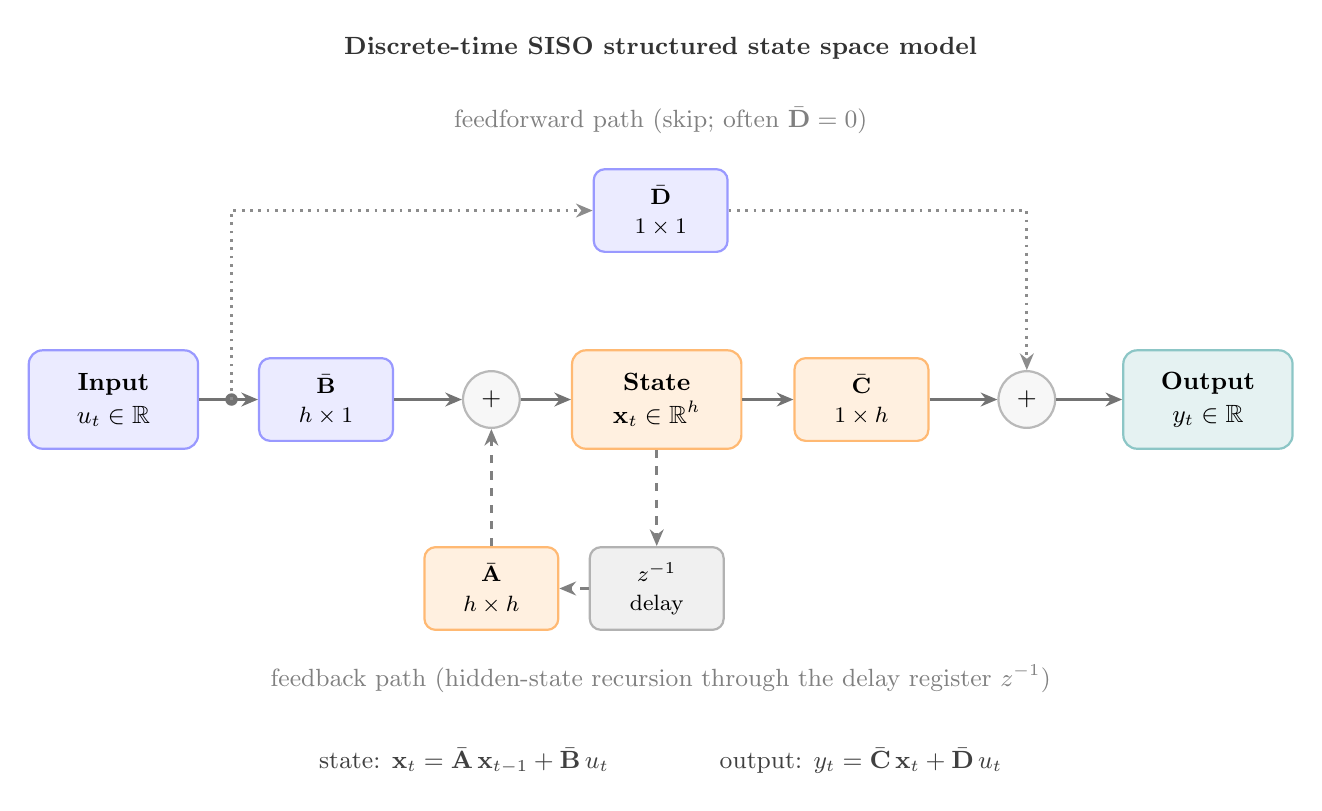
\begin{tikzpicture}[
    mainblock/.style  = {rectangle, draw=gray!55, thick, rounded corners=5pt,
                         minimum height=1.25cm, minimum width=2.15cm,
                         font=\small, inner sep=6pt, align=center},
    inblock/.style    = {mainblock, fill=blue!8,   draw=blue!40},
    outblock/.style   = {mainblock, fill=teal!10,  draw=teal!45},
    opblock/.style    = {mainblock, fill=orange!12, draw=orange!55},
    matblock/.style   = {rectangle, draw=gray!55, thick, rounded corners=4pt,
                         minimum height=1.05cm, minimum width=1.7cm,
                         font=\footnotesize, inner sep=4pt, align=center},
    matB/.style       = {matblock, fill=blue!8,    draw=blue!40},
    matC/.style       = {matblock, fill=orange!12, draw=orange!55},
    matA/.style       = {matblock, fill=orange!12, draw=orange!55},
    matD/.style       = {matblock, fill=blue!8,    draw=blue!40},
    delay/.style      = {matblock, fill=gray!12,   draw=gray!60},
    conn/.style       = {line width=1.0pt, draw=black!55,
                         -{Stealth[length=6pt, width=5pt]}},
    fbconn/.style     = {line width=1.0pt, draw=black!50, dashed,
                         -{Stealth[length=6pt, width=5pt]}},
    skipconn/.style   = {line width=1.0pt, draw=black!45, dotted,
                         -{Stealth[length=6pt, width=5pt]}},
    plus/.style       = {circle, draw=gray!55, thick, fill=gray!6,
                         minimum size=0.72cm, font=\small, inner sep=0pt},
    annot/.style      = {font=\small, text=black!50, align=center},
    eqnlbl/.style     = {font=\small, text=black!75, align=center},
    titlelbl/.style   = {font=\small\bfseries, text=black!80, align=center},
    tinytap/.style    = {circle, fill=black!55, inner sep=0pt, minimum size=4.5pt},
]

%% ============================================================
%% COORDINATES
%% ============================================================
\def\xU{0}
\def\xB{2.7}
\def\xSa{4.8}
\def\xX{6.9}
\def\xC{9.5}
\def\xSb{11.6}
\def\xY{13.9}

\def\xMid{6.95}

\def\yMain{0}
\def\ySkip{2.4}
\def\yFb{-2.4}
\def\yTitle{4.2}
\def\yCaption{-4.3}

%% ============================================================
%% MAIN-PATH NODES
%% ============================================================
\node[inblock]  (u)  at (\xU,  \yMain) {\textbf{Input}\\[1pt]$u_{t}\in\mathbb{R}$};
\node[matB]     (B)  at (\xB,  \yMain) {$\bar{\mathbf{B}}$\\[1pt]\footnotesize $h\times 1$};
\node[plus]     (s1) at (\xSa, \yMain) {$+$};
\node[opblock]  (x)  at (\xX,  \yMain) {\textbf{State}\\[1pt]$\mathbf{x}_{t}\in\mathbb{R}^{h}$};
\node[matC]     (C)  at (\xC,  \yMain) {$\bar{\mathbf{C}}$\\[1pt]\footnotesize $1\times h$};
\node[plus]     (s2) at (\xSb, \yMain) {$+$};
\node[outblock] (y)  at (\xY,  \yMain) {\textbf{Output}\\[1pt]$y_{t}\in\mathbb{R}$};

%% skip row (feedforward)
\node[matD]     (D)  at (\xMid, \ySkip)
    {$\bar{\mathbf{D}}$\\[1pt]\footnotesize $1\times 1$};

%% feedback row
\node[delay]    (z)  at (\xX,  \yFb) {$z^{-1}$\\[1pt]\footnotesize delay};
\node[matA]     (A)  at (\xSa, \yFb) {$\bar{\mathbf{A}}$\\[1pt]\footnotesize $h\times h$};

%% ============================================================
%% MAIN-PATH CONNECTIONS
%% ============================================================
\draw[conn] (u.east)  -- (B.west);
\draw[conn] (B.east)  -- (s1.west);
\draw[conn] (s1.east) -- (x.west);
\draw[conn] (x.east)  -- (C.west);
\draw[conn] (C.east)  -- (s2.west);
\draw[conn] (s2.east) -- (y.west);

%% ============================================================
%% SKIP PATH (u -> D -> s2)
%% ============================================================
\coordinate (uTap) at ($(u.east)!0.55!(B.west)$);
\node[tinytap] at (uTap) {};
\draw[skipconn] (uTap) |- (D.west);
\draw[skipconn] (D.east) -| (s2.north);

%% ============================================================
%% FEEDBACK PATH (x_t -> z^{-1} -> A -> s1)
%% ============================================================
\draw[fbconn] (x.south) -- (z.north);
\draw[fbconn] (z.west)  -- (A.east);
\draw[fbconn] (A.north) -- (s1.south);

%% ============================================================
%% PATH ANNOTATIONS (centered on \xMid, off the blocks)
%% ============================================================
\node[annot, anchor=south] at (\xMid, \ySkip + 0.85)
    {feedforward path (skip; often $\bar{\mathbf{D}}=0$)};
\node[annot, anchor=north] at (\xMid, \yFb - 0.85)
    {feedback path (hidden-state recursion through the delay register $z^{-1}$)};

%% ============================================================
%% TITLE
%% ============================================================
\node[titlelbl, anchor=south] at (\xMid, \yTitle)
    {Discrete-time SISO structured state space model};

%% ============================================================
%% EQUATION CAPTION
%% ============================================================
\node[eqnlbl, anchor=north] at (\xMid, \yCaption)
    {state: $\mathbf{x}_{t} = \bar{\mathbf{A}}\,\mathbf{x}_{t-1} + \bar{\mathbf{B}}\,u_{t}$
     \qquad\qquad
     output: $y_{t} = \bar{\mathbf{C}}\,\mathbf{x}_{t} + \bar{\mathbf{D}}\,u_{t}$};

\end{tikzpicture}
\end{document}
